\documentclass[11pt]{article}
\usepackage[utf8]{inputenc}
\usepackage[T1]{fontenc}
\usepackage{geometry}
\usepackage{amsmath}
\usepackage{amssymb}
\usepackage{enumerate}
\usepackage{amsthm}
\usepackage{amsfonts}
\usepackage{mathrsfs}
\usepackage{verbatim}
\usepackage{tikz}
\usepackage{geometry}
\usepackage{hyperref}
\usepackage{tocloft}
\usepackage{mathtools}
\usepackage[object=vectorian]{pgfornament}
\usetikzlibrary{calc,fadings,decorations.pathreplacing}
\geometry{letterpaper, portrait, margin=1in}
\allowdisplaybreaks

%% Helper macros for tikz image

\newcommand\pgfmathsinandcos[3]{%
  \pgfmathsetmacro#1{sin(#3)}%
  \pgfmathsetmacro#2{cos(#3)}%
}
\newcommand\LongitudePlane[3][current plane]{%
  \pgfmathsinandcos\sinEl\cosEl{#2} % elevation
  \pgfmathsinandcos\sint\cost{#3} % azimuth
  \tikzset{#1/.style={cm={\cost,\sint*\sinEl,0,\cosEl,(0,0)}}}
}
\newcommand\LatitudePlane[3][current plane]{%
  \pgfmathsinandcos\sinEl\cosEl{#2} % elevation
  \pgfmathsinandcos\sint\cost{#3} % latitude
  \pgfmathsetmacro\yshift{\cosEl*\sint}
  \tikzset{#1/.style={cm={\cost,0,0,\cost*\sinEl,(0,\yshift)}}} %
}
\newcommand\DrawLongitudeCircle[2][1]{
  \LongitudePlane{\angEl}{#2}
  \tikzset{current plane/.prefix style={scale=#1}}
   % angle of "visibility"
  \pgfmathsetmacro\angVis{atan(sin(#2)*cos(\angEl)/sin(\angEl))} %
  \draw[current plane] (\angVis:1) arc (\angVis:\angVis+180:1);
  \draw[current plane,dashed] (\angVis-180:1) arc (\angVis-180:\angVis:1);
}
\newcommand\DrawLatitudeCircle[2][1]{
  \LatitudePlane{\angEl}{#2}
  \tikzset{current plane/.prefix style={scale=#1}}
  \pgfmathsetmacro\sinVis{sin(#2)/cos(#2)*sin(\angEl)/cos(\angEl)}
  % angle of "visibility"
  \pgfmathsetmacro\angVis{asin(min(1,max(\sinVis,-1)))}
  \draw[current plane] (\angVis:1) arc (\angVis:-\angVis-180:1);
  \draw[current plane,dashed] (180-\angVis:1) arc (180-\angVis:\angVis:1);
}
\newcommand{\sectionline}
{\noindent
  \begin{center}
  {\resizebox{0.5\linewidth}{1ex}
  {{{
\begin{tikzpicture}
  \node (C) at (0,0){};
  \node (D) at (9,0){};
  \path (C) to [ornament=85] (D);
  \end{tikzpicture}}}}}
  \end{center}
}
\newtheorem{theorem}{Theorem}[subsection]

\theoremstyle{definition}
\newtheorem{definition}{Definition}[subsection]

\theoremstyle{definition}
\newtheorem*{definition*}{Definition}

\theoremstyle{definition}
\newtheorem{example}{Example}[subsection]

\theoremstyle{remark}
\newtheorem*{remark}{Remark}

\renewcommand{\bf}{\bfseries}
\renewcommand{\sc}{\scshape}
\renewcommand{\it}{\itshape}

\renewcommand{\bar}[1]{\mkern 1.5mu\overline{\mkern-1.5mu#1\mkern-1.5mu}\mkern 1.5mu}
\newcommand{\vectorproj}[2][]{\textit{proj}_{#1}#2}

\renewcommand\cftsecfont{\bf\sc}
\renewcommand\cftsecpagefont{\normalfont}
\renewcommand{\cftsecleader}{\cftdotfill{\cftdotsep}}
\renewcommand\cftsecdotsep{\cftdot}
\renewcommand\cftsubsecdotsep{\cftdot}

\newcommand{\Ker}{\text{Ker}}
\newcommand{\R}{\mathbb{R}}
\newcommand{\C}{\mathbb{C}}
\newcommand{\Z}{\mathbb{Z}}

\hypersetup
{pdfauthor={Kevin Cheng},
pdftitle={CO 255 W18 Course Notes},
pdfsubject={Optimization}
pdflang={English}}

\begin{document}

\begin{titlepage}
\begin{centering}
{\scshape\LARGE University of Waterloo \par}
\begin{figure}[!h]
\centering
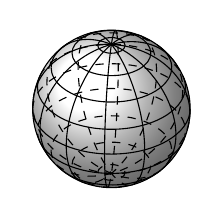
\begin{tikzpicture} % Title page sphere
\def\R{1} % sphere radius
\def\angEl{35} % elevation angle
\filldraw[ball color=white] (0,0) circle (\R);
\foreach \t in {-80,-60,...,80} {\DrawLatitudeCircle[\R]{\t}}
\foreach \t in {-5,-35,...,-175} {\DrawLongitudeCircle[\R]{\t}}
\end{tikzpicture}
\end{figure}
{\huge\bf CO 255}\\
{\scshape\Large Introduction to Optimization (Advanced)}\\
\vspace{.3cm}
{\scshape Prof. Ricardo Fukasawa~\textbullet~Winter 2018 \par}
\end{centering}
\sectionline
\tableofcontents
\sectionline
\thispagestyle{empty}
\end{titlepage}

\section{Introduction}
\subsection{Types of Optimization Problems}
Given a set $S$ and an objective function $f: S \to \R$, an optimization problem
looks like,
\begin{equation*}
\max_{\text{subject to (s.t.)}} f(x)_{x \in S}
\end{equation*}
which means to find some $x* \in S$ such that $f(x) \leq f(x*)$ for all $x \in
S$. Here, $S$ is called the ``Feasible Region'', and a point $\bar x \in S$ is
called a ``feasible solution'' and $f(\bar x)$ is called the ``objective
value''.
\begin{definition}
For some feasible region $S$, $x*$ is an \underline{optimal solution} if for all
$x \in S$ that $f(x) \leq f(x*)$.
\end{definition}
We can use different notation like
\begin{equation*}
\max \{f(x) : x\in S \}
\end{equation*}
or
\begin{equation*}
\max_{x \in S} f(x).
\end{equation*}
Also, there is a correspondence with \underline{minimization problems} as,
\begin{equation*}
\max_{x \in S} f(x) = -\bigg( \min_{x \in S} -f(x) \bigg) 
\end{equation*}
A number of problems can arise,
\begin{itemize}
\item $S = \emptyset$ (This problem is always \underline{infeasible})
\item If for all $a \in \R$, there always exists some $\bar x \in S: f(\bar x)
> a$ (This problem is \underline{unbounded})
\item $\max_{x < 1} x$ (Here, an optimal solution does not exist)
\end{itemize}
\begin{definition}
A \underline{supremum} is defined as \begin{equation*}
\sup{f(x):x \in S} =
\begin{cases}
- \infty,& \text{, if infeasible}\\
+ \infty,& \text{, if unbouded}\\
\min_{f(x) \leq \lambda,\>\text{for all } x \in S}\lambda, &\text{, otherwise}\\
\end{cases}
\end{equation*}
\end{definition}
\begin{definition}
The \underline{infimum} can be defined as
\begin{equation*}
\inf_{x \in S} f(x) = - \sup_{x \in S} -f(x)
\end{equation*}
\end{definition}
So now by replacing maximization problems with the supremum (and minimization
problems with infimum), we would never fall into the case where ``an optimal
solution doesn't exist'' as long as we consider the supremum (or infimum). In
other words, if the problem is feasible and unbounded, we can always find an
optimal solution.

\subsection{Linear Programming (LP)}
Given an $m \times n$ matrix A, and some $\vec b \in \R^m $, we can consider the
feasible region defined by
\begin{equation*}
S =\{\vec x \in \R^n: A\vec x \leq \vec b\}.
\end{equation*}
We can also consider some $f(\vec x) = \vec{c}^T \vec x$ for some $\vec c \in \R^n$.
\begin{definition}
For some vectors $\vec u,\vec v \in \R^n$, we compare them by component-wise comparison.
We say \underline{$\vec u \leq \vec v$} if and only if $u_i \leq v_i$ for all
$i = 1, \dots, n$. 
\end{definition}
\begin{remark}
$\vec u \not\leq \vec v$ does not imply $\vec u > \vec v$. For example,
\begin{equation*}
\begin{pmatrix}
1 \\ 2
\end{pmatrix}
,
\begin{pmatrix}
2 \\ 1
\end{pmatrix}
\end{equation*}
\end{remark}
\begin{remark}
Strict inequalities are \underline{not} allowed.
\end{remark}
\begin{definition}
A \underline{polyhedron} is
\begin{equation*}
\{\vec x \in \R^n: A\vec x \leq \vec b\}.
\end{equation*}
In other words, a polyhedron is the intersection of finitely many linear
inequalities.
\end{definition}
\begin{example}
Suppose $n$ products and $m$ resources.
\begin{itemize}
\item $b_i$ units of resources $i$, for all $i = 1, \dots, m$
\item $c_j$ per unit profit of producing product $j$, for all $j = 1, \dots, n$
\item Producing $d$ units of $j$ consumes $a_{ij}$ units of resource $i$, for
all $i = 1,\dots,m$
\end{itemize}
We define decision variables $x_j$ for all $j = 1,\dots,n$ to represent amount
of product $j$ produced. We can consider the linear program,
\begin{align*}
\max &\sum^n_{j=1} c_jx_j\\
\text{s.t.} & \sum^n_{j=1} a_{ij}x_j \leq b_i,\> \forall i = 1,\dots,m\\
& \vec x \geq \vec 0
\end{align*}
\end{example}

\subsection{Determining Infeasibility}
The problem is quite easy if $n=1$. We simply determine if the polyhedron is
empty. So the idea is to reduce the problem from $n$ variables to $n-1$
variables, and eventually to the 1-dimensional case.
\begin{definition}
Suppose we have some feasible region $S$ defined as,
\begin{equation*}
S \coloneqq \{(\vec x, \vec y) \in \R^n \times \R^p: A\vec x + G\vec y \leq b\}
\end{equation*}
then the \underline{orthogonal projection of $S$ onto $\vec x$} is defined as
\begin{equation*}
\vectorproj[\vec x]{S} := \{\vec x \in S: \exists \vec y\> \text{such that }
(\vec x, \vec y) \in S\}.
\end{equation*}
\end{definition}
The idea now is to determine if $S$ is feasible by determining if
$\vectorproj[x_1,\dots,x_{n-1}]{S}$ is feasible. In order to do so, we have 3
more definitions to break down our LP\@. To do so, we need a few definitions.\\

Consider the following set,
\begin{equation*}
M \coloneqq \{1 ,\dots, m\} 
\end{equation*}
then, we have the following 3 definitions:
\begin{equation*}
M^+ \coloneqq \{i \in M : a_{in} > 0\}
\end{equation*}
\begin{equation*}
M^- \coloneqq \{i \in M : a_{in} < 0\}
\end{equation*}
\begin{align*}
M^\circ &\coloneqq M \setminus (M^+ \cup M^-)\\
&= \{i \in M: a_{in} = 0\}
\end{align*}
Now, we can break down our LP into 3 parts. All three of these parts break down
perfectly into the following theorem:
\begin{theorem}
There exists $\bar{x}_n$ such that $\vec x = (\bar{x}_1, \dots, \bar{x}_n)$
satisfies
\begin{equation}
\sum^{n-1}_{j=1} \frac{a_{ij}}{a_{in}} + x_n \leq \frac{b_i}{a_{in}}, \forall i
\in M^+
\end{equation}
\begin{equation}
\sum^{n-1}_{j=1} -\frac{a_{ij}}{a_{in}} - x_n \leq -\frac{b_i}{a_{in}}, \forall i
\in M^-
\end{equation}
and
\begin{equation}
\sum^{n-1}_{j=1}a_{ij}x_j \leq  b_i, \forall i \in M^\circ
\end{equation}
if and only if $(\bar{x}_1, \dots, \bar{x}_{n-1})$ satisfies (3), which is
\begin{equation*}
\sum^{n-1}_{j=1} -\frac{a_{ij}}{a_{in}} - x_n \leq -\frac{b_i}{a_{in}}, \forall i
\in M^\circ
\end{equation*}
\begin{equation}
\sum^{n-1}_{j=1}\Big(\frac{a_{ij}}{a_{in}} - \frac{a_{kj}}{a_{kn}} \Big)x_j
\leq \frac{b_i}{a_{in}} - \frac{b_i}{a_{kn}} , \forall i \in M^+, \forall k \in
M^-
\end{equation}
\begin{remark}
This gives a condition that allows us to reduce LPs from $n$ dimensions down to
$n-1$ and the new LP is given by (4).
\end{remark}
\end{theorem}
\end{document}

